\chapter{Spark-SIFT性能测试和分析}
\section{实验环境}
本文构建了一个包含7台PC机的PC集群作为Spark-SIFT系统的性能测试和分析实验平台,实验平台集群的主要配置参数如下:
\begin{compactenum}
\item 集群总体配置7台PC,其中1台master,6台worker;Spark的版本为2.0.0,集群的管理模式采用Spark原生的standalone模式。
\item Master节点配置为:处理器AMD APU,内存为16GB,硬盘为1TB,操作系统为Ubuntu 14.04;
\item Slave节点配置为:处理器Intel,内存12GB,硬盘为1TB,操作系统为Ubuntu 14.04;
\end{compactenum}

因为实验中,我们还选取了GPU作为对比试验,GPU的配置为NVIDIA GTX760,CUDA 4.0。

在测试数据集上,在测试key-value图片描述性能时,我们从ImageNet 2012\upcite{Imagenet}中随机选择了8个不同规模的图片集作为测试输入,分别是500 KB(8),70 MB (530),140 MB (1003),280 MB (1833),1 GB(8719 张),2 GB(15024张),4 GB (28721)和11 GB(78492张),圆括号中为图片文件的数量。在测试分割式图片特征提取算法及shuffle-efficent特征提取算法时,本文采用作者平时搜集到的高清图片作为测试数据集,这是图片大都是2M以上,最大有4M多。
\section{实验结果与分析}
在实验设计上,本文首先分析key-value图片描述方式,分割式特征提取算法以及Shuffle-efficient特征提取算法这三种优化策略的性能。最后本文将Spark-SIFT系统分别和SIFT的单机版本,GPU版本对比,分析性能的差异。
\subsection{key-value图片描述方式}
在key-value图片描述方式的性能分析上,本文和binaryFile以及objectFile两种方式进行对比,对比它们在加载不同的数据集大小图片所要耗费的时间,如图\ref{fig:data_loadPerformance}所示,测试时,采用的并行任务数是100个,当加载的图片数据较小时,三种加载方式并没有什么较大的差距,比如加载140M时,key-value 图片描述方式的加载时间为6S,binaryFile加载方式的加载时间为8S,objectFile加载方式的加载时间为8S。当加载的规模增大时,key-value方式的加载性能就提升的较为明显,在加载11G图片数据集时,key-value方式的加载时间为39S,binaryFile加载方式的加载时间为102S,objectFile加载方式的加载时间为234S,key-value图片描述方式的加载速度相对于binaryFile方式为2.6倍,相对于objectFile方式为6倍。因此在加载众多小文件时,本文设计的key-value图片描述方式大大的提高了加载的性能。

\begin{figure}[htp]
\centering
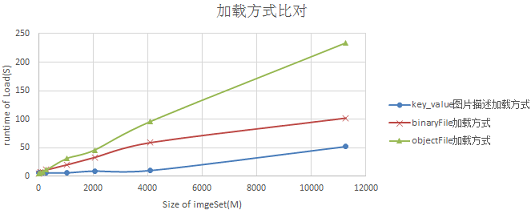
\includegraphics{data_loadPerformance}
\caption{三种图片集合的加载性能比较}
\label{fig:data_loadPerformance}
\end{figure}
因为key-value方式是存在一个序列化预处理过程的,为了设计更加有说服力,本文也测试了序列化预处理时间占总处理时间的比例,同时如图\ref{fig:data_keyValue_ratio} 所示,随着图片集规模的增加,序列化时间占总处理时间的比例也在不断减小。当图片规模小于280 MB 时,序列化时间占总处理时间的比例较高,超过了10\%;随着图片集的不断增大,序列化时间占总运行时间的比重会略微下降,对于11 GB 的图片集合,序列化时间为300s,约占总处理时间的8\%。所以在处理大规模数据时,预处理并不会占用太多时间。
\begin{figure}[htp]
\centering
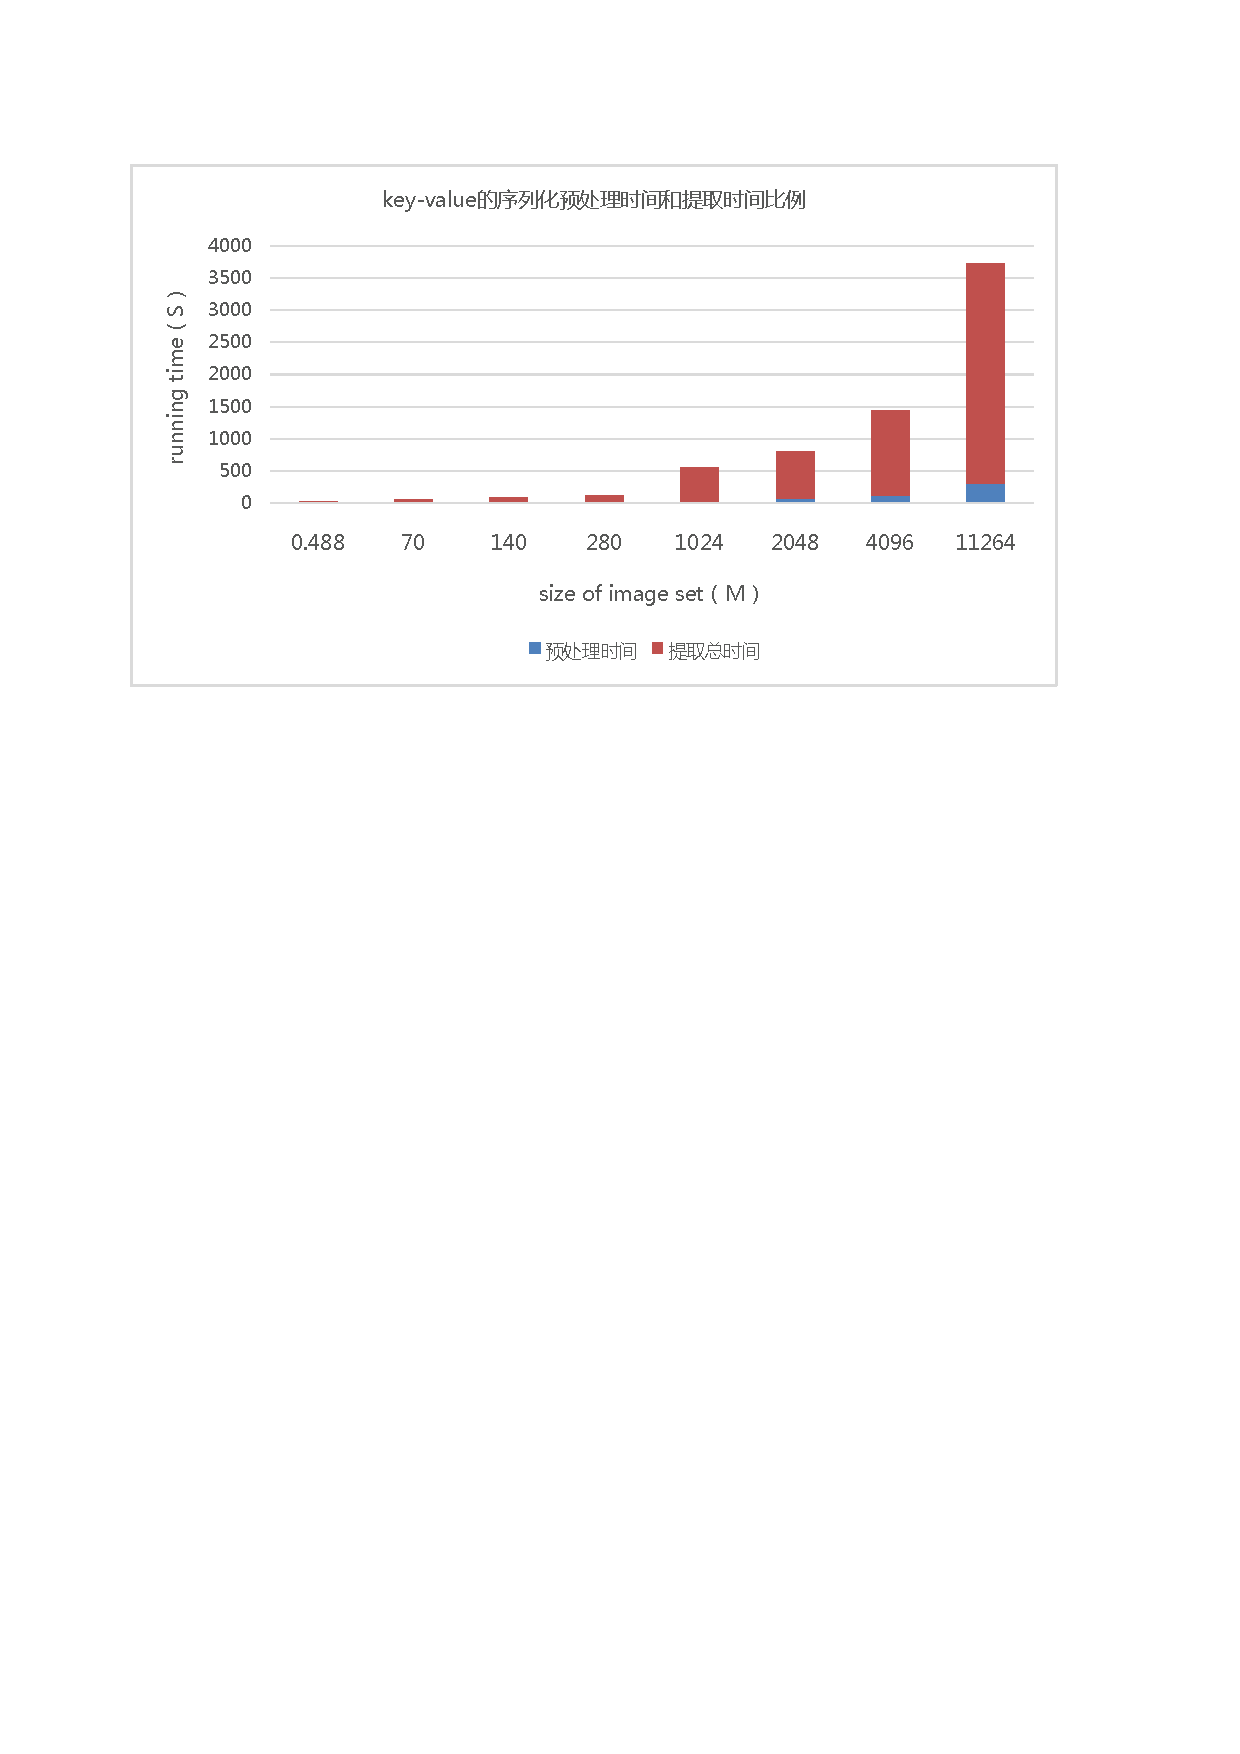
\includegraphics{data_keyValue_ratio}
\caption{key-valuede的预处理时间和提取时间比例}
\label{fig:data_keyValue_ratio}
\end{figure}

\subsection{分割式特征提取算法}
在测试图片分割策略的优化效果时,我们采用了总容量为480 MB的图片集合作为输入。集合中有280 MB的``小``图片,其大小在100到200KB 之间,而其余200 MB则是``大``图片,图片大小在2\~4MB之间。当图片大小的差距增大时(例如KB与GB,或MB与GB),这种优化带来的性能提升将更加明显。图\ref{fig:data_seg_speed}描述了在不同的分割大小下,Spark-SIFT完成特征处理的时间。如图7所示,分割大小越小,提取的速度越快,例如在10×10的分割大小下,提取全部480 MB 图片特征的时间仅为210 秒。但是如图\ref{fig:data_seg_accuracy}所示,分割大小越小,提取出的特征点的误差也越大,例如在10×10的分割大小下,误差率约为12\%。因此,综合提取速度和提取精确率两个因素,本文选取500×500作为分割大小。
\begin{figure}[htp]
\centering
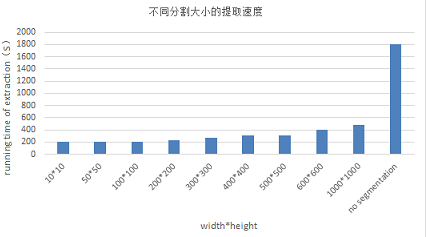
\includegraphics{data_seg_speed}
\caption{不同分割大小的提取速度}
\label{fig:data_seg_speed}
\end{figure}

\begin{figure}[htp]
\centering
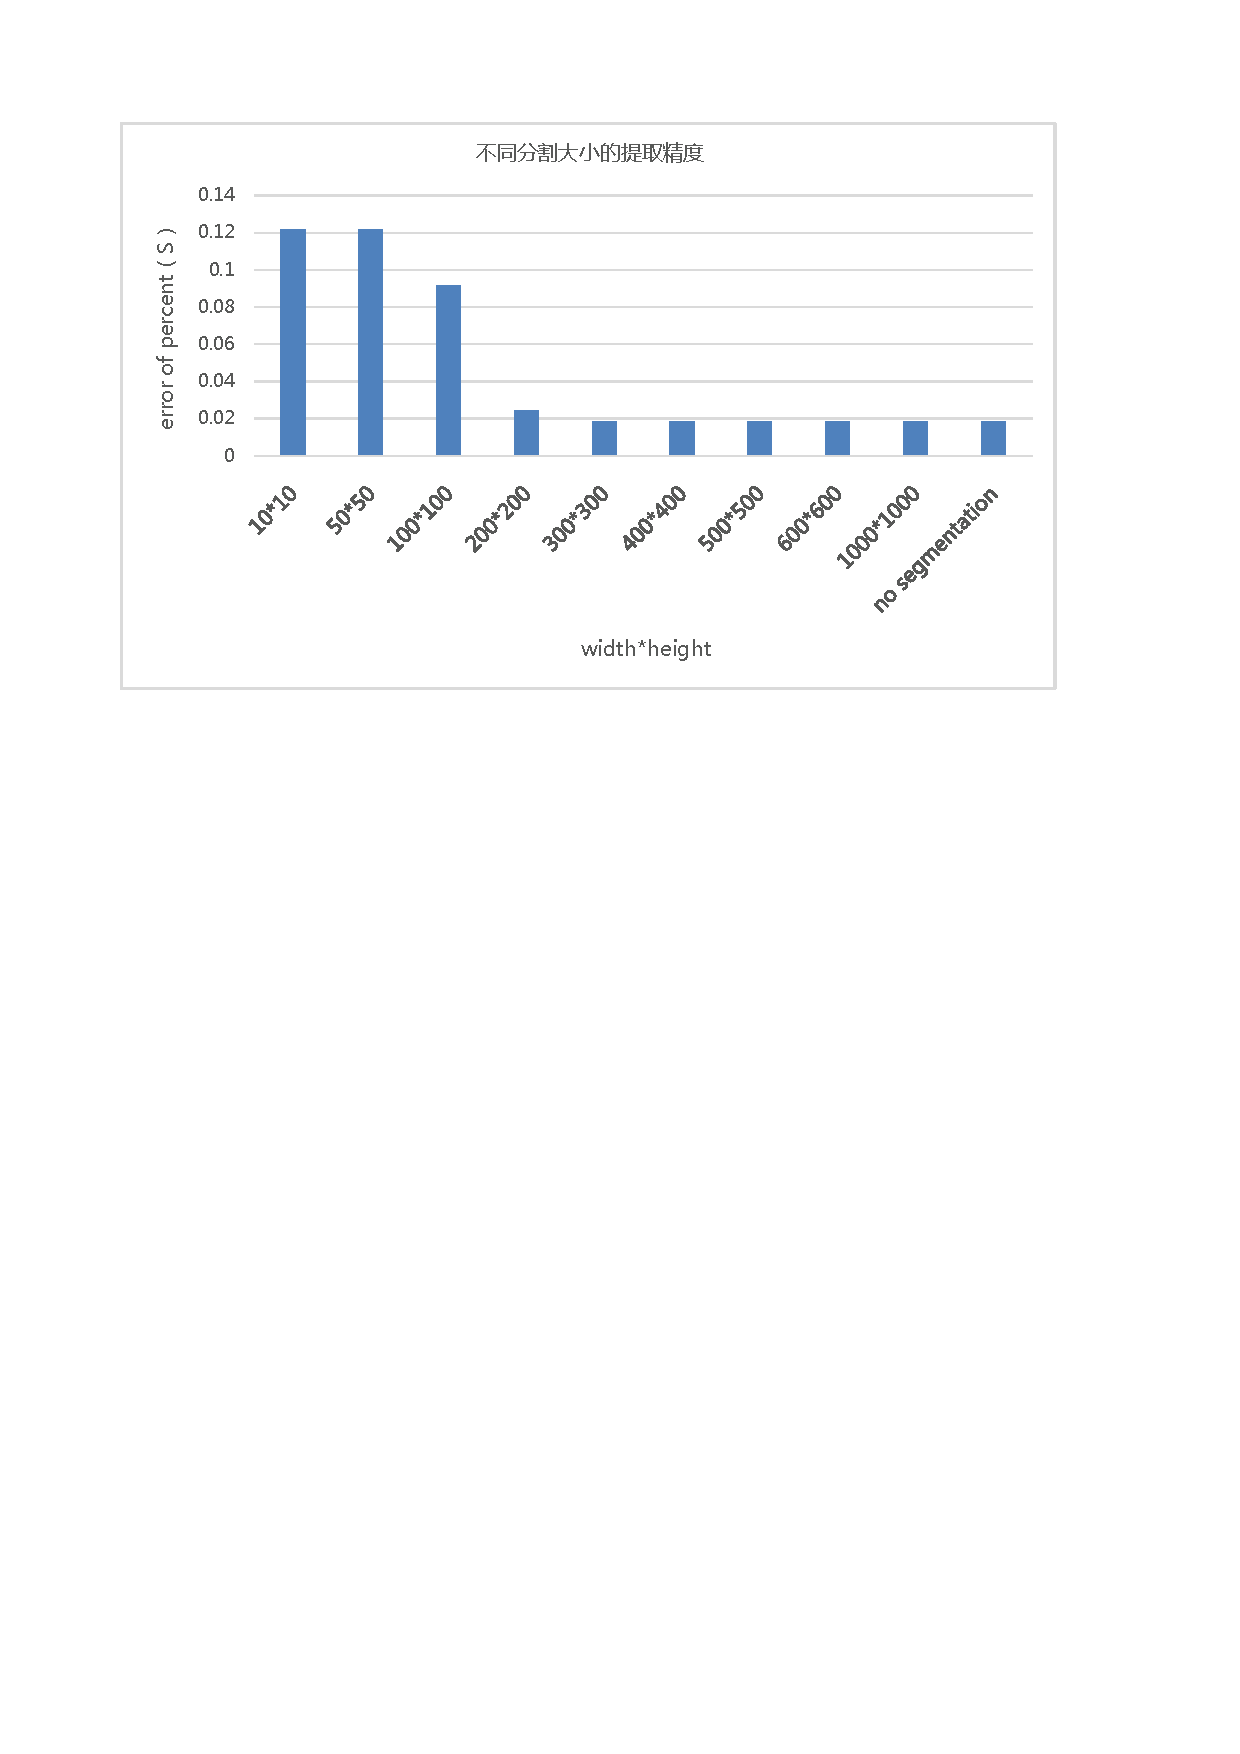
\includegraphics{data_seg_accuracy}
\caption{不同分割大小的提取精度}
\label{fig:data_seg_accuracy}
\end{figure}

\subsection{Shuffle-efficient特征提取算法}
在验证Shuffle-efficient特征提取算法的有效性上,本文将采用高效分区策略的Shuffle-efficient提取算法和采用Hash分区策略的分割式提取算法进行比较,在不同的测试图片数据集下对比它们在reduceByKey 步骤上所耗费的时间,以及Shuffle的数据量大小。如图\ref{fig:data_Partition}所示,本文对高效分区策略和Hash分区策略分别测试了3.2G及6.8G两组图片数据集。当数据集为3.2G时,采用高效分区策略的子块收集时间为169.087S,采用Hash分区策略的收集时间为199.742S,时间减少了大约30S,收集性能提高了约15\%,当测试规模增大到6.8G时,高效分区的收集时间为383.532S,Hash分区的收集时间为546.007S,收集性能提高了29.7\%,说明图片数据集越大时,高效的分区策略对于分割式特征提取算法越能减少收集的网络开销。
\begin{figure}[htp]
\centering
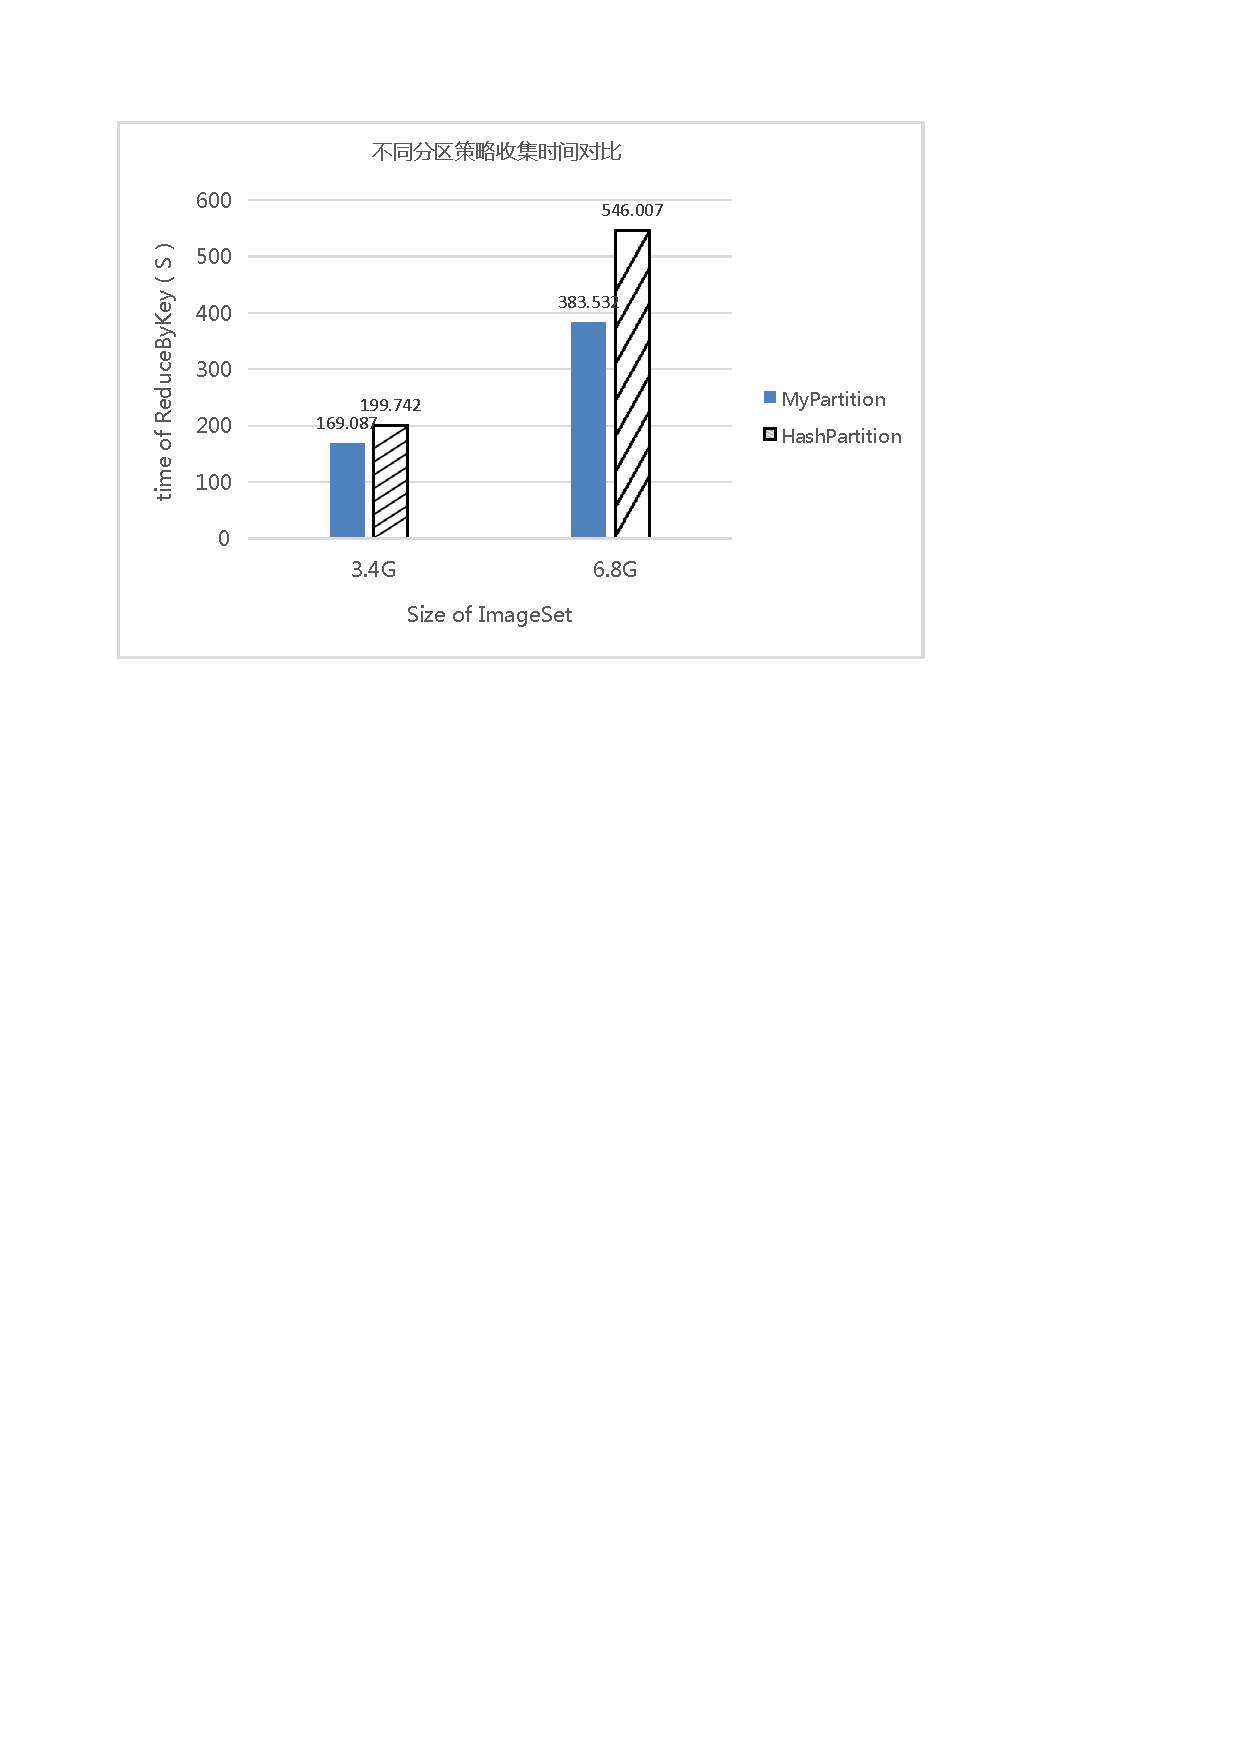
\includegraphics{data_Partition}
\caption{两种分区策略在收集子块的时间开销}
\label{fig:data_Partition}
\end{figure}

\subsection{系统综合性能对比}
从图\ref{fig:data_fourWays}可以看出,对于500 KB的图片集,GPU的处理时间最短,在不到1s的时间就完成了所有图片的特征提取;无论是否采用序列化,Spark-SIFT的特征提取速度比单机还要慢,这是因为在图片数较少时,Spark进行任务分配和数据收集等操作的开销占据了总运行时间中的很大一部分,此时无法体现出Spark的性能优势。当图片集大小为70 MB 时,Spark-SIFT的特征速度已经优于单机版本了——序列化方式下的提取时间为44.8s,而单机的提取时间则为470.71s,获得了大约10.5倍的性能加速。GPU版本的处理时间为44.98s,与序列化Spark-SIFT基本相同。随着图片集大小的不断增加,Spark-SIFT在提取时间上的优势也越来越明显。例如,在4 GB的输入规模下,Spark-SIFT的处理时间为1319.25s,单机版本的处理时间为28020.03s,速度已经相差了接近20倍,GPU版本的处理时间为2671.18s,是Spark-SIFT的两倍。因此,对于GB级别以上的图片规模,Spark-SIFT体现出较大的性能优势。
\begin{figure}[htp]
\centering
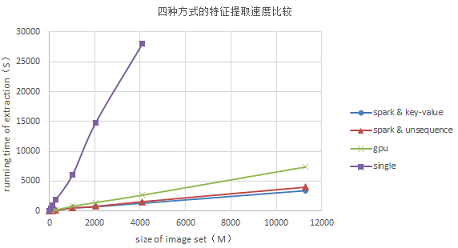
\includegraphics{data_fourWays}
\caption{四种方式的特征提取速度比较}
\label{fig:data_fourWays}
\end{figure}

总的说来,当图片集大小为GB量级时,与单机版本相比,Spark-SIFT能够带来大约21倍的性能加速,GPU版本能带来大约10倍的性能加速,如图\ref{fig:data_seg_speedup} 所示。
\begin{figure}[htp]
\centering
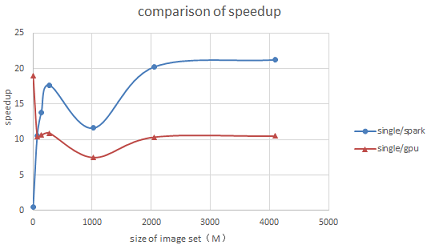
\includegraphics{data_seg_speedup}
\caption{spark和单机,GPU和单机加速度比较}
\label{fig:data_seg_speedup}
\end{figure}

图\ref{fig:data_spark_gpu}进一步对比了Spark-SIFT与GPU两个版本的性能,分析了访问磁盘的开销对处理时间的影响。如果没有将结果写到文件中,GPU版本的提取速度快于Spark-SIFT,快了大约0.5倍;当要将结果保存在文件中时,GPU版本的提取速度比Spark-SIFT慢了约1 倍。由此可见,访问磁盘的开销在大规模特征提取时还是相当大的。
\begin{figure}[htp]
\centering
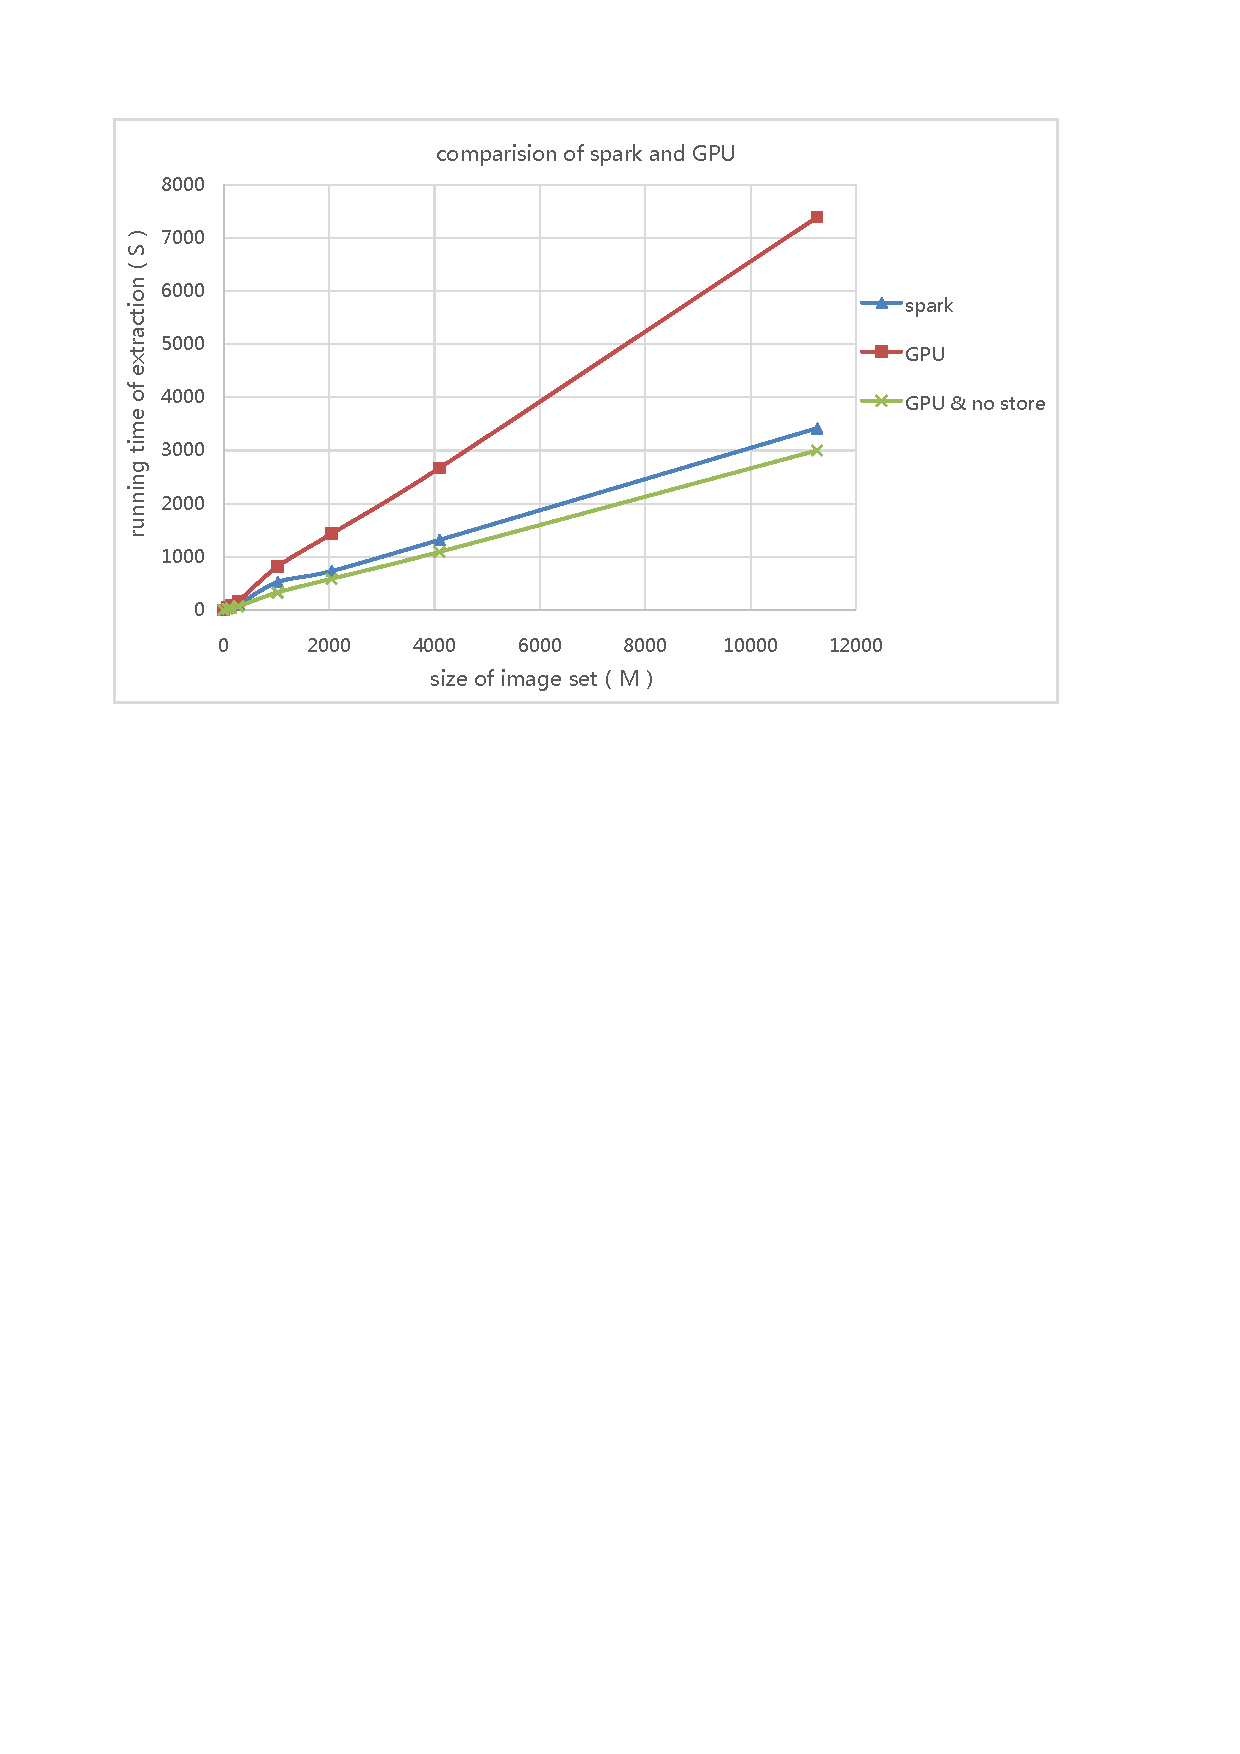
\includegraphics{data_spark_gpu}
\caption{spark和GPU两种方式比较}
\label{fig:data_spark_gpu}
\end{figure}
\section{本章小结}
本章分析Spark-SIFT系统的综合性能以及针对其提出的三种优化方案。从实验数据来,Spark-SIFT系统在处理GB级别以上的图片数据集时,速度明显快于单机的处理速度,加速比优化GPU,从而达到了设计的预期目标。

